\documentclass[a4paper,12pt,twoside,openright,titlepage]{book}

%Additional packages
\usepackage[utf8]{inputenc}
\usepackage[T1]{fontenc}
\usepackage[dutch,english]{babel}
\usepackage{imakeidx}
\usepackage{syntonly}
\usepackage[official]{eurosym}
\usepackage{graphicx}
\graphicspath{ {./images/} }
\usepackage{wrapfig}
\usepackage{float}
\usepackage{xurl}
\usepackage{hyperref}
\hypersetup{colorlinks=true, linkcolor=blue, citecolor=blue, filecolor=blue, urlcolor=blue, pdftitle=, pdfauthor=, pdfsubject=, pdfkeywords=}
\usepackage{tabularx}
\usepackage[table]{xcolor} % Table colors
\usepackage{scrextend}
\addtokomafont{labelinglabel}{\sffamily}
\usepackage{listings}
\usepackage{adjustbox}
\usepackage{color}
\usepackage{csquotes}

% Define colors
\definecolor{ashgrey}{rgb}{0.7, 0.75, 0.71}

% Listing style
\lstset{
  backgroundcolor=\color{ashgrey}, % choose the background color; you must add \usepackage{color} or \usepackage{xcolor}; should come as last argument
  basicstyle=\footnotesize,        % the size of the fonts that are used for the code
  breakatwhitespace=true,          % sets if automatic breaks should only happen at whitespace
  breaklines=true,                 % sets automatic line breaking
  extendedchars=true,              % lets you use non-ASCII characters; for 8-bits encodings only, does not work with UTF-8
  frame=single,	                   % adds a frame around the code
  rulecolor=\color{black},         % if not set, the frame-color may be changed on line-breaks within not-black text (e.g. comments (green here))
  keepspaces=true,                 % keeps spaces in text, useful for keeping indentation of code (possibly needs columns=flexible)
  columns=fullflexible,		   % make copy and paste possible
  showstringspaces=false,          % if true show spaces in strings adding particular underscores
  showspaces=false,                % if true show spaces everywhere adding particular underscores; it does not override 'showstringspaces'
}

% Uncomment for production
% \syntaxonly

% Style
\pagestyle{headings}

% Turn on indexing
\makeindex[intoc]

% Define document
\author{D. Leeuw}
\title{NTP}
\date{\today\\v.0.8.0}

\begin{document}
\selectlanguage{dutch}

\maketitle

\copyright\ 2023 Dennis Leeuw\\

\begin{figure}

\includegraphics[width=0.3\textwidth]{CC-BY-SA-NC.png}
\end{figure}

\bigskip

Dit werk is uitgegeven onder de Creative Commons BY-NC-SA Licentie en laat anderen toe het werk te kopi\"eren, distribueren, vertonen, op te voeren, en om afgeleid materiaal te maken, zolang de auteurs en uitgever worden vermeld als maker van het werk, het werk niet commercieel gebruikt wordt en afgeleide werken onder identieke voorwaarden worden verspreid.


%%%%%%%%%%%%%%%%%%%
%%% Introductie %%%
%%%%%%%%%%%%%%%%%%%

\frontmatter
\chapter{Over dit Document}
\section{Leerdoelen}
Dit document gaat over ethernet. Het leert je wat ethernet is. Om meer te weten te komen over wat er op je netwerk gebeurt maak je ook kennis met de tools: \texttt{arp} en \texttt{wireshark}.

Na het bestuderen van dit document heb je een basis kennis van ethernet, weet je wat het adres-formaat is van ethernet en kan je informatie over het netwerk opvragen via verschillende tools.

In de praktijk opdrachten leer je om je eigen kabel te maken en deze te testen. Tevens maak je je eigen Wi-Fi netwerk.

\section{Voorkennis}
Er wordt van de lezer verwacht dat deze kennis heeft van de volgende onderwerpen:
\begin{itemize}
\item TCP/IP
\item CMOS en BIOS tijd
\end{itemize}


%%%%%%%%%%%%%%%%%
%%% De inhoud %%%
%%%%%%%%%%%%%%%%%
\tableofcontents

\mainmatter
\chapter{Inleiding}
NTP, het Network Time Protocol, is een protocol dat over het Internet en lokale TCP/IP netwerken gebruikt wordt om te zorgen dat alle systemen dezelfde tijd hebben. NTP is een application layer protocol. Werkstations gebruiken NTP-servers om hun klokken mee te synchroniseren.



\chapter{De lokale tijd}
Je computer houdt de tijd bij\index{Computer!tijd}\index{Tijd!Computer}. Standaard is dat een functie van het CMOS\index{CMOS}, dus ook als de computer uit staat wordt de tijd bijgehouden. De klok van je computer is afhankelijk van het kristal\index{kristal}\index{Computer!kristal} op het moederbord. Elk kristal is uniek en heeft dus ook een unieke frequentie. Computers lopen na verloop van tijd niet meer gelijk met de tijd in de wereld. Dit geldt overigens niet alleen voor computers ook klokken lopen na verloop van tijd voor of achter. De vraag die ontstaat is: wat is dan die tijd in de wereld?

Tegenwoordig gebruiken we atoomklokken\index{Atoomklok} om de tijd van de wereld in uit te drukken. Zie voor de werking van een atoomklok deze link: \url{https://www.quantumuniverse.nl/hoe-werkt-een-atoomklok}.

We hebben afspraken gemaakt om te zorgen dat iedereen op tijd op zijn werk is. We hebben de aarde opgedeeld in tijdzones\index{Tijdzones}. Binnen een tijdzone is de tijd hetzelfde is. Zo is het in Nederland, Belgi\"e, Frankrijk en Spanje altijd op hetzelfde moment 12:00 uur. In het Verenigd Koninkrijk is het een uur later dan bij ons en in Rusland is het een uur vroeger dan bij ons, zij zitten in een andere tijdzone. Tijzones lopen van de Noordpool naar de Zuidpool en binnen zo'n zone houden we dezelfde tijd aan. De nul-lijn\index{Nul-lijn} voor de lengte graad ligt over Greenwich\index{Greenwich} in het Verenigd Koninkrijk. In Nederlands zitten we dus op +1 en in Rusland op +2 ten opzichte van die nul-lijn. Als we de andere kant op gaan van de nul-lijn dan komen we in New York en zitten we op -5 uur ten opzichte van de nul-lijn. Een factor die het hele verhaal nog iets complexer maakt is het gebruik van de zomer-\index{Zomertijd} en wintertijd\index{Wintertijd}.

Er is dan ook voor gekozen om \'e\'en universele tijd te hebben en daaruit de lokale tijd te berekenen. Die universele tijd wordt UTC\index{UTC} (Coordinated Universal Time\index{Coordinated Universal Time}). Als je wil weten waarom de afkorting afwijkt van de naam verwijzen we je graag naar de Wikipedia-pagina \url{https://en.wikipedia.org/wiki/Coordinated_Universal_Time}. De voorganger van UTC is GMT\index{GMT} ofwel Greenwich Mean Time\index{Greenwich Mean Time}.



\chapter{De netwerk tijd}
De tijd wordt bijgehouden door atoomklokken. Het is onhandig om een atoomklok in te bouwen in elke computer. De meest eenvoudige oplossing is om de tijd uit te zenden via de lucht en deze weer op te vangen met een ontvanger. Dat gebeurd met de DCF77 Tijdseinzender\index{DCF77 Tijdseinzender} in Duitsland. Wekkers, stationsklokken en elk ander apparaat kan dit signaal ontvangen en zorgen dat zijn interne klok gesynchroniseerd is met deze klok. Een ontvanger voor deze zender inbouwen in een computerkast is lastig want de standaard kasten zijn van staal en ontvangen dus geen radiosignalen van buitenaf, dat is precies de reden waarom ze van staal zijn om verstoring van buitenaf te minimaliseren. Er zou natuurlijk een ontvanger ingebouwd kunnen worden met een antenne buiten de kast, dat is een mogelijke oplossing en die oplossingen bestaan ook.

Daar tegenwoordig bijna elke computer aan een netwerk hangt is het handiger om de tijd via het netwerk te versturen. We moeten dan natuurlijk wel rekening houden met de vertragingen op het netwerk en daar compensatie berekeningen op loslaten, maar met wat goede wil en een paar hele slimme programmeurs moet dat te doen zijn. De oplossing die we tegenwoordig kennen heet NTP\index{NTP} (Network Time Protocol\index{Network Time Protocol}).

Op het Internet zijn er tijdservers die op een manier de atoomkloktijd doorzetten naar het Internet. Als iedereen tegen deze servers aan zou praten dan zou er al snel niet voldoende bandbreedte zijn. Om dit probleem op te lossen, de oplossing voor dit probleem is het gebruik van zogenaamde NTP-pools\index{NTP-pool}\index{Pool}. Vele servers samen vormen een pool waarbinnen de tijd gesynchroniseerd wordt, door tegen zo'n pool te praten wordt de load op het netwerk verdeeld. Je kan zelf ook een NTP-server opzetten en je aansluiten bij zo'n pool zodat je onderdeel wordt van de oplossing. Er zijn natuurlijk wel enkele eisen waaraan je moet voldoen om mee te doen met zo'n pool. E\'en van die eisen is dat de server 24/7 beschikbaar moet zijn.

Tijdservers op het Internet kunnen hun klok synchroniseren met een atoomklok\index{Atoomklok}, met het DCF77\index{DCF77} tijdsignaal of met GPS\index{GPS}. Al deze bronnen leveren een accurate tijdsbron.



\chapter{NTP}
NTP is een protocol waarmee computers in een netwerk hun interne klok kunnen synchroniseren. NTP maakt hiervoor gebruik van UDP port 123.


\section{NTP Servers}

\begin{wrapfigure}{l}{0.33\textwidth} %this figure will be at the left
    \centering
    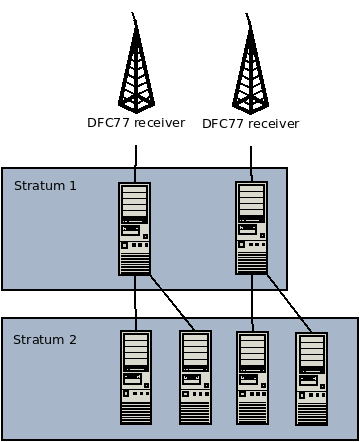
\includegraphics[width=0.33\textwidth]{Stratums}
\end{wrapfigure}

NTP is een hi\"erarchische structuur opgedeeld in stratums\index{Stratum}. Een \textquote{stratum 1} server is een server die direct gekoppeld is aan een referentieklok (atoomklok, DCF77 of GPS). De referentie klokken zijn stratum 0. Een server die zijn tijd haalt van een stratum 1 server heet een stratum 2 server. Een tijdserver die zijn tijd haalt van een stratum 2 server heet dan logischerwijs een stratum 3 server. Dit gaat zo door tot maximaal stratum 16.

Hoe hoger het stratum nummer hoe meer de tijd afwijkt van de tijd van de referentieklok. Middels berekeningen en onderlinge synchronisatie van servers in een bepaald stratum wordt deze onnauwkeurigheid zoveel mogelijk beperkt.


\section{NTP Client}
NTP gaat ervan uit dat de vertraging op het netwerk te meten is en dat deze gelijk is voor de heen- en de terugweg:
\begin{enumerate}
\item Client stuurt packet naar server en zet daarin een timestamp van zijn tijd (T1)
\item De server registreert de tijd dat het packet binnen komt (T2)
\item De server stuurt het packet weg op (T3) (Het packet van de server bevat T1, T2 en T3)
\item De client ontvangt het packet op T4 en heeft nu 4 tijdstippen.
\end{enumerate}
De vertraging over de heenweg is T2-T1, de vertraging over de terugweg is T4-T3. Omdat we ervan uit gegaan dat de netwerkvertraging symmetrisch is moet een verschil tussen T2-T1 en T4-T3 te maken hebben met het verschil in de klok. Dit verschil in de klok noemen we de offset en kan berekend worden via:
\[ offset = (T2 - T1 + T3 - T4)/2 \]
De offset kan dus positief of negatief zijn afhankelijk van of onze klok achter of voor staat ten opzichte van de serverklok.

Laten we in een tabel een rekenvoorbeeld maken. We zeggen dat de tijd op de server 10 seconden voor staat ten opzichte van de client, de network delay 20 seconden is en we beginnen op T1=0:
\begin{center}
\begin{tabular}{ |l|c|c|c|c|c|c| }
\hline
Actie & Tijd op client & T1 & T2 & T3 & T4 & Tijd op server \\
\hline
Client verstuurt T1 & 00 & 00 & - & - & - & 10 \\
\hline
Server ontvang T1 & 20 & 00 & 30 & - & - & 30 \\
\hline
Server verstuurt T1,T2,T3 & 22 & 00 & 30 & 32 & - & 32 \\
\hline
Client ontvangt packet & 42 & 00 & 30 & 32 & 42 & 52 \\
\hline
\end{tabular}
\end{center}
Hieruit kunnen we via de eerder genoemde formule de offset berekenen:
\[ offset = (30 - 0 + 32 - 42)/2 = 10 \]
en dat klopt precies met wat we al wisten, namelijk dat de server 10 seconden voorloopt op onze klok. We moeten onze klok dus 10 seconden vooruit zetten.



%%%%%%%%%%%%%%%%%%%%%
%%% Index and End %%%
%%%%%%%%%%%%%%%%%%%%%
\backmatter
\printindex
\end{document}

%%% Last line %%%
